\begin{pr}
$g(x)=\P[x<X\leq c]=F_X(c)-F_X(x)$.\\
$\then F_Y(y)=\P[Y\leq y]=\P[g(X)\leq y]=\P[F_X(c)-F_X(X)\leq y]=\P[F_X(X)\geq F_X(c)-y]=1-\P[F_X(X)\leq F_X(c)-y]\overtext{ by the definition of CDF }=1-F_X(c)+y$.\\
$\cuz g(x)\geq0$ and $g(x)\leq\P[X\leq c]=F_X(c)$.\\
$\so F_Y(y)=\begin{cases}
0\text{, if }y<0\\
1-F_X(c)+y\text{, if }0\leq y\leq F_X(c)\\
1\text{, if }y\geq F_X(c)\\
\end{cases}$.\\
Note that $F_Y(y)$ is not necessarily continuous since $\P[Y=0]=\P[X\geq c]=1-F_X(c)$.\\
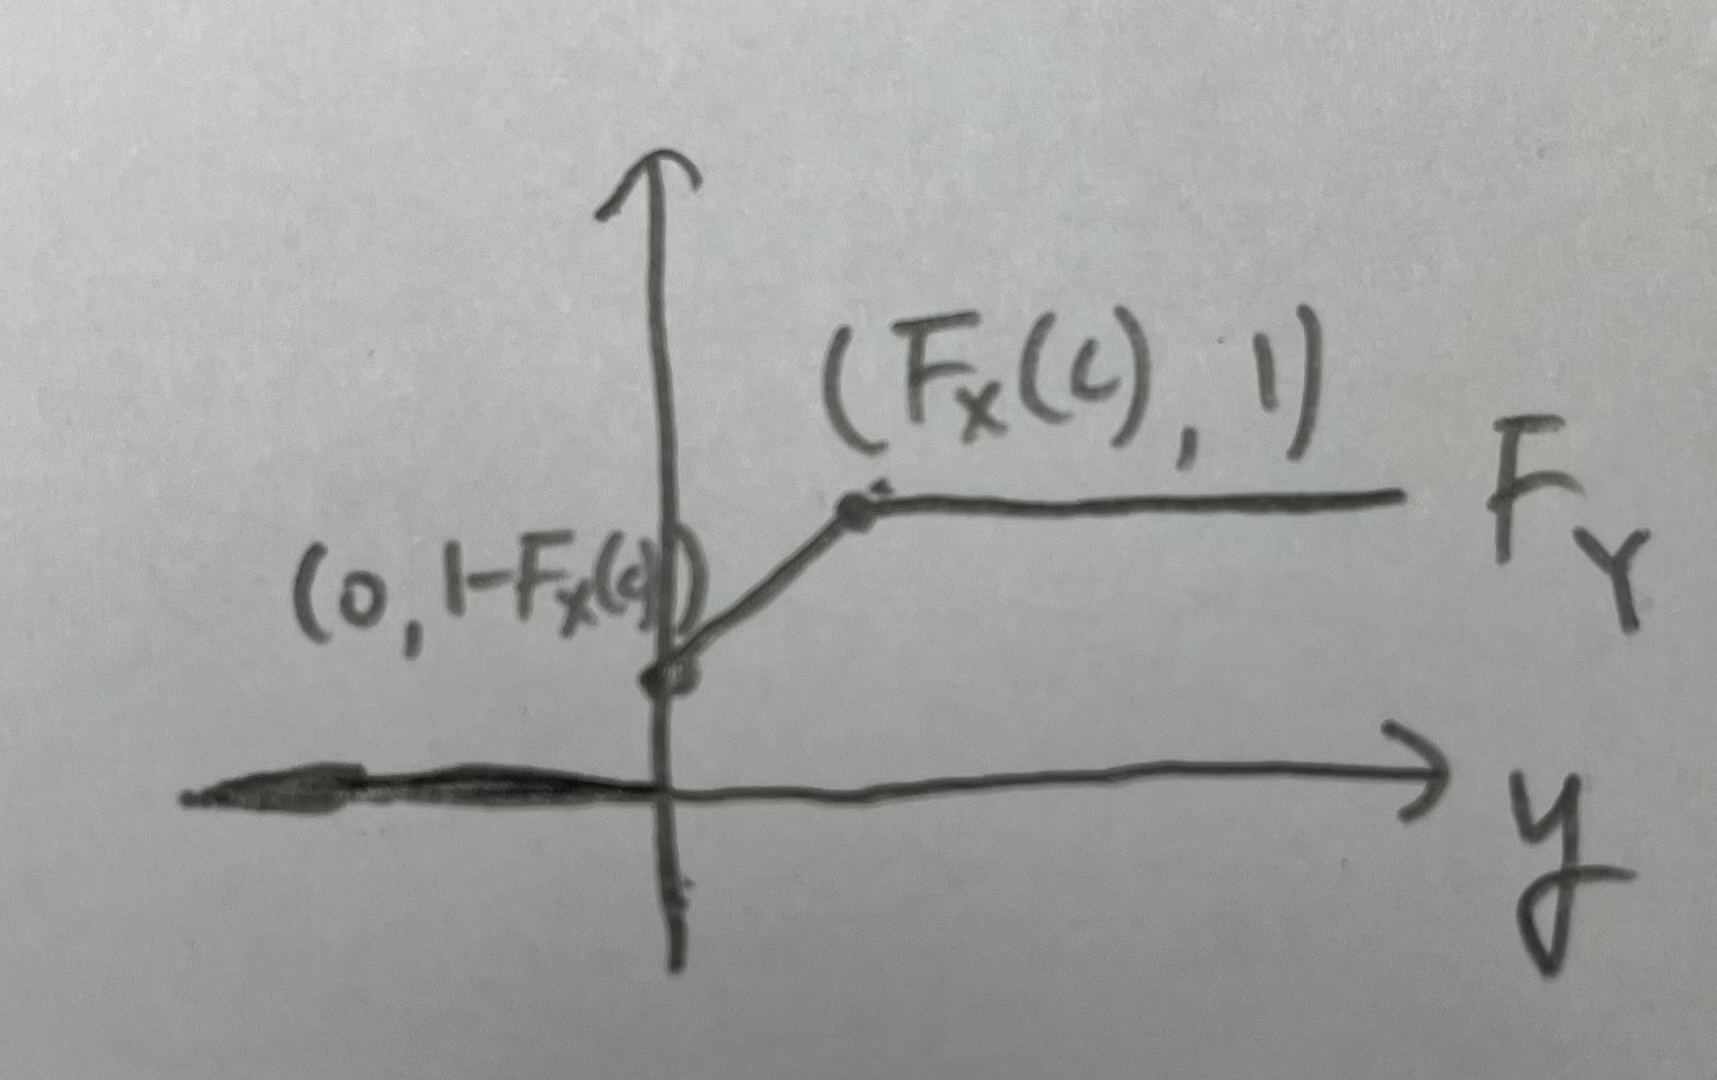
\includegraphics[width=6cm]{6.JPG}
\end{pr}
